\documentclass[conference]{IEEEtran}
\IEEEoverridecommandlockouts
% The preceding line is only needed to identify funding in the first footnote. If that is unneeded, please comment it out.
\usepackage{cite}
\usepackage{amsmath,amssymb,amsfonts}
\usepackage{algorithmic}
\usepackage{graphicx}
\usepackage{textcomp}
\usepackage{xcolor}
\usepackage{float}
\usepackage{makecell}
\usepackage{url}
\def\BibTeX{{\rm B\kern-.05em{\sc i\kern-.025em b}\kern-.08em
    T\kern-.1667em\lower.7ex\hbox{E}\kern-.125emX}}
\begin{document}

\title{Design of optical codirectional coupler for integrated silicon photonics devices}

\author{\IEEEauthorblockN{Otávio M. Paiano}
\IEEEauthorblockA{\textit{Instituto de Física ``Gleb Wataghin"} \\
\textit{Universidade Estadual de Campinas}\\
Campinas, Brazil \\
o185284@dac.unicamp.br}
}

\maketitle

\begin{abstract}
The efficient design of a photonic silicon on insulator co-directional coupler is discussed for three different approaches: coupled mode theory (CMT), supermode (SM) analysis and finite-difference time-domain (FDTD) numerical simulations. The final parameters for the coupler are  a coupling length of $7.2\ \mu\text{m}$ and a gap of $87$ nm. Divergencies between CMT, SM and FDTD approaches are discussed. 
\end{abstract}

\begin{IEEEkeywords}
Silicon, photonics, coupler, codirectional, design.
\end{IEEEkeywords}

\section{Introduction}
The design of nanophotonic structures is an important building block for industrial applications and scientific advances based on photonic integrated devices. A key component of photonic devices are co-directional couplers. In this work, we analyze three different approaches for designing a co-directional coupler made of silicon ($\text{Si}$, refractive index of $3.48$) waveguides immersed in silica ($\text{SiO}_2$, refractive index of $1.45$). 

The approaches employed are coupled mode theory (CMT), supermode analysis (SM) and Finite-Difference Time-Domain (FDTD). While the first two methods rely on the modal solution of the device's waveguides, the FDTD method provides a solution of the full Maxwell equations on time domain, and therefore also take into account the adiabatic separation between the waveguides on the input and output ports of the device (the s-bends of the waveguides).

\begin{table}[ht]
\caption{Requirements for the directional coupler.}
\begin{center}
\begin{tabular}{|l|c|l|c|}
\hline
\textbf{Parameter description} & \textbf{\textit{Symbol}}& \textbf{\textit{Value}}& \textbf{\textit{Fixed/variable}} \\
\hline\hline
Core refractive index$^{\mathrm{a}}$ & $n_1$ & 3.48 & Fixed \\
\hline
Cladding refractive index$^{\mathrm{b}}$ & $n_0$ & 1.45 & Fixed \\
\hline
Waveguides' width & $w$ & 500 nm & Fixed \\
\hline
Waveguides' height & $h$ & 220 nm & Fixed \\
\hline
Central wavelength & $\lambda_0$ & 1560 nm & Fixed  \\
\hline
Bandwidth & $\Delta\nu$ & 5 THz & Fixed  \\
\hline
Gap between waveguides & $g $ & $> 0$ nm & Variable \\
\hline
Coupling length & $L_c $ & $< 10 \ \mu\text{m}$ & Variable \\
\hline
Minimum power transfer & $ T_{min} $ & $\geq -0.3 $ dB & Variable \\
\hline
\multicolumn{4}{l}
{\makecell[l]{$^{\mathrm{a}}$Silicon refractive index for $\lambda_0 \approx 1550$ nm. \\ $^{\mathrm{b}}$Silica refractive index for $\lambda_0 \approx 1550$ nm.}}
\end{tabular}
\label{tab:1}
\end{center}
\end{table}


\begin{figure}[ht]
\centerline{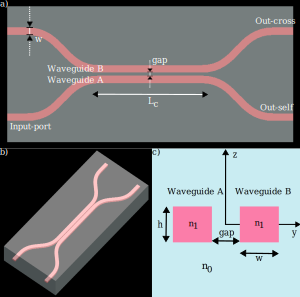
\includegraphics[width=0.8\linewidth]{projeto2/figs/device_props.pdf}}
\caption{Device geometry and parameters as specified in Table \ref{tab:1}: a) Cross-section of the device for $z=0$. b) 3D rendering of the device. c) cross-sectional view of the device in a plane perpendicular to the propagation direction $x$.}
\label{fig:device}
\end{figure}



A summary of the design requirements for waveguide geometry, materials, wavelength, and other constraints are given in Table \ref{tab:1}. In Fig. \ref{fig:device}, we show a schematic of the device. 





\section{Methodology}
Firstly, the system is simulated using CMT and SM approaches. After initial estimates for $L_c$ by means of CMT and SM, a fine-tuning is performed using FDTD.



\subsection{Coupled mode theory}
Coupled mode theory is a perturbation method that can be used to describe the interactions between two propagation modes, which under the assumption of weak coupling between the modes on different waveguides allows for the computation of power transfer between the waveguides along the propagation direction. The power exchange between the waveguides is achieved by the evanescent coupling provided that the overlap integral between the input mode and the mode on the other waveguide is non-zero. 

In this work, the waveguides have a rectangular cross-sectional shape and the mode of interest in both waveguides is the fundamental $E_{11}^x$ mode (also known as the fundamental quasi-TE mode). Therefore, the overlap integral is non-zero and the excitation of the fundamental mode by evanescent coupling is attainable. For this particular case, the directional coupling coefficient, $\kappa$, can be approximated by solving the transcendental equations that lead to the effective index of a single waveguide\cite{okamoto}.

Since the fundamental quasi-TE optical modes in both waveguides have equal effective indices due to identical waveguide geometries, the phase-mismatch $\delta$ is zero:
\begin{equation}
    \delta = \beta_a - \beta_b = 0.
\end{equation}
Therefore, maximum power transfer efficiency may be achieved provided the device has a sufficiently long coupling distance. Thus, the coupling length is given by\cite{okamoto}:
\begin{equation}
    L_c = \dfrac{\pi}{2\kappa}.
\end{equation}

\subsection{Supermode analysis}

The supermode analysis is based on the modal solution for a cross-section of the device in the propagation direction in an area encompassing both waveguides in the coupling region. From the effective indices obtained from the modal solutions, the coupling length  the supermode analysis is given by\cite{okamoto}
\begin{equation}
    L_c = \dfrac{\pi}{\beta_e - \beta_o} = \dfrac{\lambda_0}{2\Delta n},
\label{eq:Lc_supermodes}
\end{equation}
where $\beta_e$ and $\beta_o$ are, respectively, the propagation constants of the even and odd modal solutions of the fundamental quasi-TE modes and $\Delta n$ is the difference between even and odd modes' refractive indices. The modal solution may be numerically obtained by Finite Element Methods (FEM) or Finite Difference Eigenmode (FDE). From the eigenvalues (the effective indices), the quantity $\Delta n$ was computed, leading to the estimations of the coupling length by means of Eq. \ref{eq:Lc_supermodes}.


\begin{figure}[ht]
\centerline{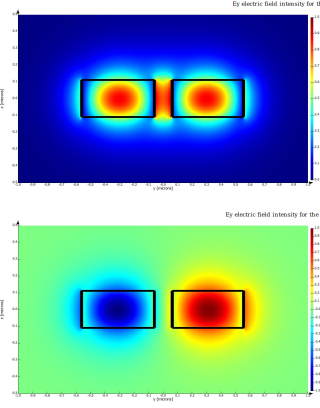
\includegraphics[width=0.9\linewidth]{projeto2/figs/supermodes_even_odd_gap120nm_1560nm.pdf}}
\caption{Supermodes' electric field intensity in the $y$ direction (quasi-TE modes) for $g=120$ nm and $\lambda_0 = 1560$ nm. The upper image is the even mode and the lower image is the odd mode.}
\label{fig:supermodes}
\end{figure}

\subsection{FDTD simulations}
A crucial step of the design process is overlooked by the two previous analysis: the continued coupling along the adiabatic separation region between the two waveguides after the coupling segment. The s-bend shape that separates the two waveguides before and after the coupling region must be taken into account in the final design of the device. For this purpose, FDTD simulations are employed to fine-tune the device and verify that the final specifications align with the design requirements. To reduce the long computational time required for a full 3D simulation, the effective index method, which collapses the 3D structure into an equivalent 2D structure of slab waveguides.

\section{Results}
To ensure the requirement of minimum transmission of $-0.3$ dB for the bandwidth of $\Delta\nu = 5 $ THz we simulate all quantities for at least two more wavelengths beyond the central wavelength $\lambda_0$: $\lambda_- \approx 1540$ nm, which corresponds to the wavelength $\lambda_0$ shifted by a frequency of $+\Delta\nu /2$ and $\lambda_+ \approx 1580$ nm, which corresponds to the wavelength $\lambda_0$ shifted by a frequency of $-\Delta\nu /2$.


All data and code used to generate the figures were made public by the author as a Github repository\cite{my_git}.

\subsection{FDTD}
To optimize the device, a sweep was employed for the gap values for a fixed value of the coupling length of $L_c = 7.2 \mu\text{m}$. After achieving the optimal gap value of $g=87$ nm, a sweep on the wavelength was performed to obtain the transmission for the cross and self output ports for each wavelength. For the desired bandwidth, the transmission is shown to be at least $\sim -0.1 $ dB  (Fig. \ref{fig:transmission}).
\begin{figure}[H]
\centerline{\includegraphics[width=0.99\linewidth]{projeto2/figs/z-slice-power.pdf}}
\caption{  Power transfer between waveguides for the optimized device ($g=87$ nm and $L_c = 7.2\ \mu\text{m}$) for wavelength $\lambda_0$.}
\label{fig:z_slice_power}
\end{figure}

\subsection{CMT and SM analysis}
From Fig. \ref{fig:Lc_vs_gap}, the main insight is the behavior of the required coupling length as a function of the gap and the wavelength. The wavelength dependence is explained as follows: higher values of $\lambda$ result in less confined modes, which ``leak" more into the cladding and therefore increase the integrand of the overlap integral. Thus, the mode coupling coefficient of the directional coupler, $\kappa$, increases. Similarly, the coupling length increases as the gap widens since the overlap integral between the modes in waveguides A and B diminishes. 

\begin{figure}[ht]
\centerline{\includegraphics[width=0.85\linewidth]{projeto2/figs/Lc_vs_gap__sweep_freq__cmt_vs_sm.pdf}}
\caption{Required coupling length for maximum transfer of power ($L_c$) as function of the gap between the waveguides for five different wavelengths for both, CMT and SM. The interval between $1540$ nm and $1580$ nm covers a frequency band of $\sim 5$ THz, as required by the project constraints.}
\label{fig:Lc_vs_gap}
\end{figure}




\begin{figure}[ht]
\centerline{\includegraphics[width=0.85\linewidth]{projeto2/figs/power_vs_z.pdf}}
\caption{Normalized power transfer between the waveguides as a function of distance. The gap for this system is $g=75$ nm and the wavelength is $1560$ nm. The other specifications follow the requirements of Table \ref{tab:1}.}
\label{fig:power_vs_z}
\end{figure}

For a single waveguide, the effective index has been found to be $\approx 2.47$ using the FDE method.





\section{Discussion}


\begin{figure}[ht]
\centerline{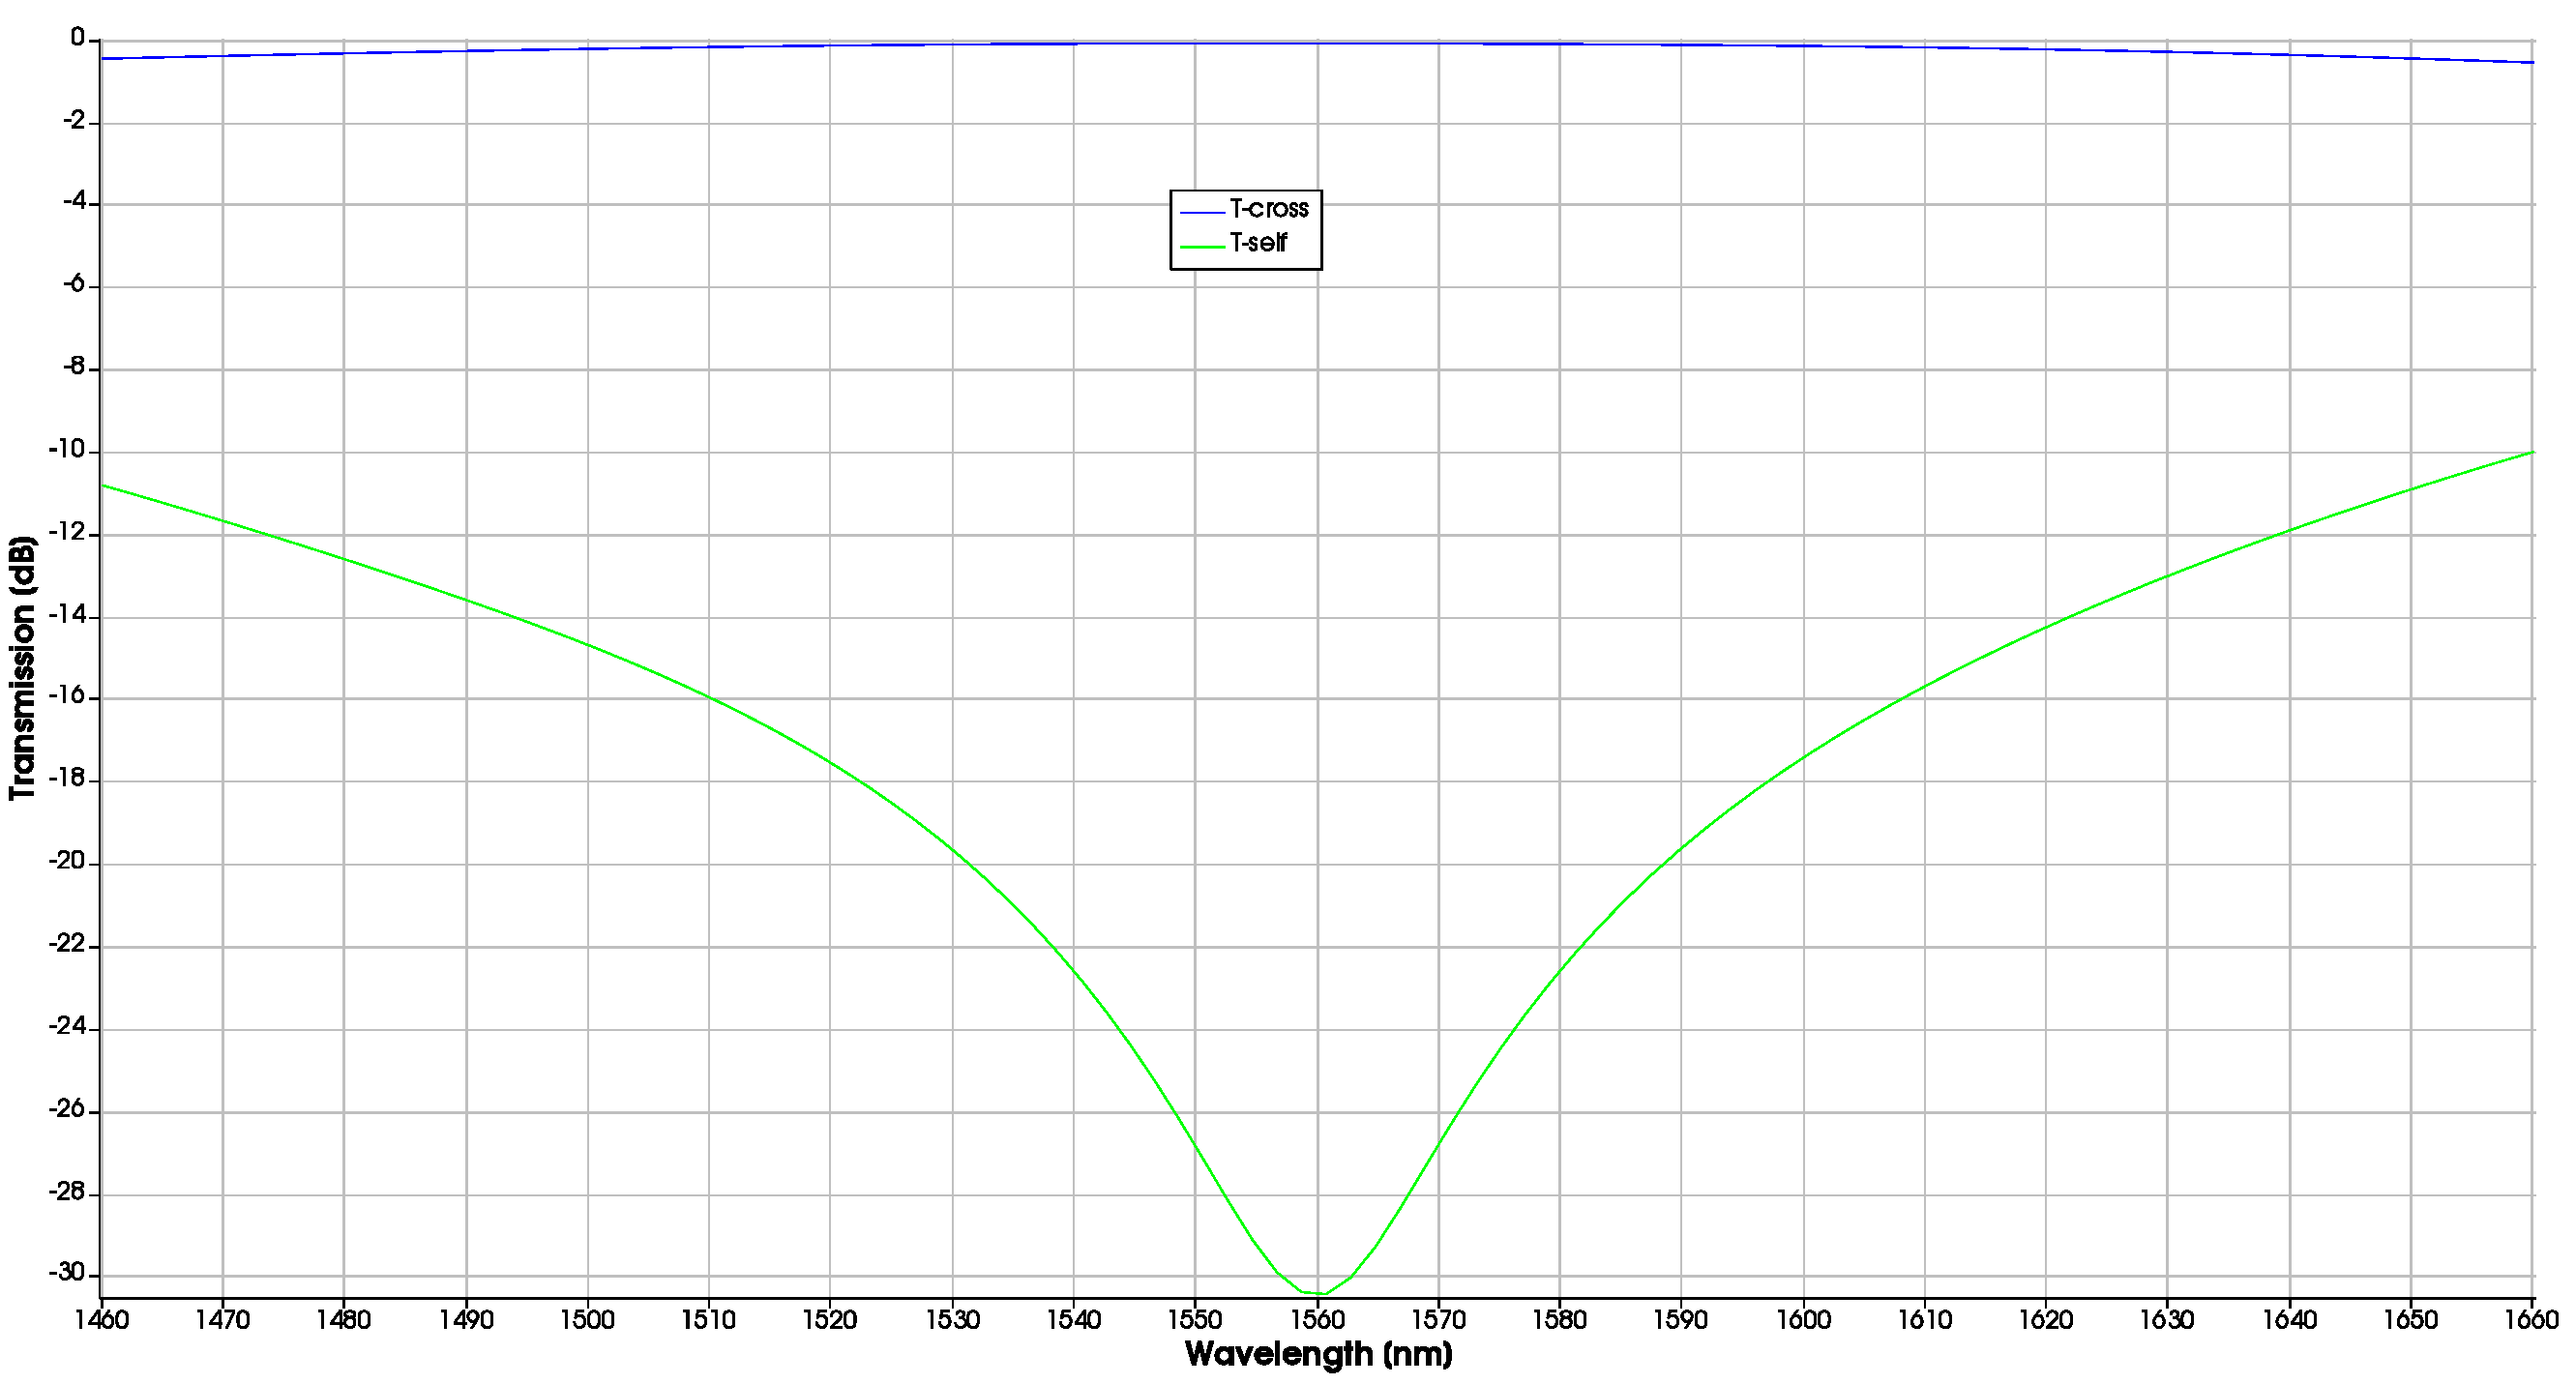
\includegraphics[width=0.9\linewidth]{projeto2/figs/transmission-gap87nm-Lc7.2microm.pdf}}
\caption{ Transmission for cross and self output ports for $g=87$ nm and $L_c = 7.2\ \mu\text{m}$.}
\label{fig:transmission}
\end{figure}




\subsection{Robustness to fabrication errors}
Given that there are many possible configurations which satisfy the project requirements, the final device specifications are determined by the parameter configuration that makes the device more robust against fabrication errors. Therefore, a longer $L_c$ is preferred, since it increases the power transfer tolerance due to fabrication errors in the coupling length.

\subsection{A comparison between CMT and SM}
CMT explained the results more effectively than SM, as it aligned more closely with FDTD simulations: values of $g$ and $L_c$ calculated from FDTD are closer to those of CMT than SM. On the other hand, when considering the remanescent coupling in the s-bend region of the device, the effective coupling length has a higher value than the reported value of $L_c = 7.2 \mu\text{m}$. Therefore, there is a margin of error to be considered from the FDTD simulations for the value of $L_c$, which could explain the divergencies between the FDTD and the CMT and SM results. However, between CMT and SM, for which the effective coupling length is precisely $L_c$, the origin of the discrepancies is unknown. However, both approaches converge for small gap values, as seen in Fig. \ref{fig:Lc_vs_gap}.

\begin{table}[ht]
\caption{Specifications of the optimized directional coupler.}
\begin{center}
\begin{tabular}{|l|c|l|}
\hline
\textbf{Parameter} & \textbf{\textit{Symbol}}& \textbf{\textit{Value}} \\
\hline\hline
Gap between waveguides & $g $ & $ 87 $ nm  \\
\hline
Coupling length & $L_c $ & $ 7.2 \ \mu\text{m}$  \\
\hline
Minimum power transfer & $ T_{min} $ & $\geq -0.1 $ dB  \\
\hline
\multicolumn{3}{l}

\end{tabular}
\label{tab:final_specifications}
\end{center}
\end{table}



\section{Conclusion}
The design of a co-directional coupler was efficiently simulated by means of CMT, SM and FDTD analysis. The requirements were fully satisfied, with transmissions of at least $-0.1$ dB even at the edges of the bandwidth. The final parameters were $g=87$ nm, which yields a coupling length of $L_c = 7.2 \mu\text{m}$ from the FDTD simulation.

\section*{Acknowledgment}
O. M. P. gratefully acknowledge professors Gilliard and Hugo for their support and insightful lectures. 

\begin{thebibliography}{00}
\bibitem{okamoto} Katsunari Okamoto, ``Fundamentals of Optical Waveguides (Second Edition)", Academic Press, ISBN 9780125250962 (2006).

\bibitem{my_git} O. M. Paiano, IE766-projeto2, (2025), GitHub repository, \url{https://github.com/ompaiano/IE766-projeto2}.

\end{thebibliography}
\vspace{12pt}

\end{document}
